\subsection{Block Ciphers}
\begin{defn}
A \textbf{block cipher} is a deterministic cryptographic algorithm that operates on fixed-size blocks of data, typically \( n \) bits, using a symmetric key to perform encryption or decryption. It transforms a plaintext block of size \( n \) bits into a ciphertext block of the same size through a series of reversible, structured operations, and vice versa.


\end{defn}
\begin{figure}[h!]
    \centering
    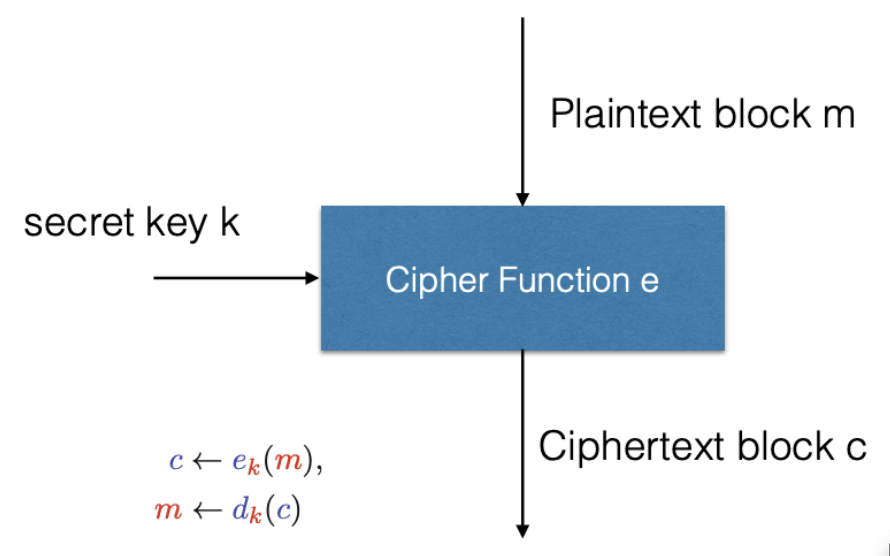
\includegraphics[width=0.5\textwidth]{img/blockcipher.png}
    \caption{Block Cipher}
    \label{fig:block_cipher}
\end{figure}

where
\begin{itemize}
    \item $m \in \{0,1\}^n$ is the plaintext block,
    \item $k \in K$ is the secret key, chosen from key space K,
    \item $e$ is the encryption function,
    \item $d$ is the decryption function,
    \item $c \in \{0,1\}^b$ is the ciphertext block.
\end{itemize}

\subsubsection{Properties of Block Ciphers}
\begin{enumerate}
    \item Input Data Block: Plaintext is divided into equal-sized blocks.
    \item Encryption/Decryption: Each block undergoes multiple transformations (substitution, permutation, and mixing) to produce ciphertext.
    \item Key: A symmetric key is applied in multiple \emph{rounds} to ensure security.
    \item Padding: If the last block of plaintext is smaller than the block size, padding is added.
    \item Modes of Operation3: Block ciphers work with data larger than one block by using modes like:
    \begin{itemize}
        \item ECB (Electronic Codebook)
        \item CBC (Cipher Block Chaining)
        \item GCM (Galois/Counter Mode)
    \end{itemize}
\end{enumerate}

Block ciphers are typically \emph{64 bits} (in DES), \emph{128 bits} (in AES) or more (in modern ciphers). They should act like a \emph{pseudorandom permutation} (PRP).

\begin{defn}
A \textbf{pseudorandom permutation} (PRP) is a function that defines a bijective (one-to-one and onto) mapping between input and output spaces, such that it is computationally indistinguishable from a truly random permutation when the key is unknown. 
\end{defn}

In order to limit the advantage of the adversary, the key space is kept very large (e.g. $Adv \ 1/|K|$). A block cipher is a \emph{building block} for designing a cipher (a PRP). A block cipher with a \emph{Mode of Operation} is a cipher. The goal is to design an IND-CCA secure cipher.

\subsubsection{Design}
DES and AES are iterated block ciphers. They \emph{repeat a simple round function}. The round $r$ can be fixed or variable. The more rounds, the higher the security of the cipher.
\begin{itemize}
    \item In each round, a round key, derived from the key $k$, is used (by key scheduling algorithm)
    \item The round function should be \emph{invertible}; for decryption the round keys are used in reverse order
    \item In DES: the round is invertible but not the round function
    \item In AES: both the round and the round function are invertible
\end{itemize}

\begin{defn}
    The \textbf{confusion-diffusion} paradigm  is a fundamental design principle for secure cryptographic systems, particularly block ciphers.
    \begin{itemize}
        \item \textbf{Confusion:} Confusion ensures that the relationship between the key and the ciphertext is highly complex, making it difficult for an attacker to infer the key, even if they have access to multiple plaintext-ciphertext pairs. Split the block into smaller blocks and apply a
        substitution on each block.
        \item \textbf{Diffusion:} Diffusion ensures that the influence of a single bit of plaintext (or key) spreads widely over the ciphertext, so that changes in input affect many output bits.  Mix permutations so that local change can effect the
        whole block.
    \end{itemize}
\end{defn} \label{def:confusion_diffusion}

\begin{defn}
    A \textbf{substitution-permutation network} (SPN) is a design model for block ciphers. It consists of a series of linked operations, including substitution, permutation, and key mixing. It is a direct implementation of defintion \ref{def:confusion_diffusion}.
\end{defn}




\subsubsection{The Avalanche Effect}
A small change in the input must affect every bit of the output. This is called the \emph{avalanche effect}. It is a desirable property of block ciphers.
\begin{enumerate}
    \item The S-boxes are designed such that 1 bit effects at least 2 bits in the output of the boxes
    \item The mixing permutations are designed
\end{enumerate}

In principle, you need at least 7 rounds for a good diffusion. \Comment{why?}

\subsection{Feistel Ciphers}

\subsection{Data Encryption Standard (DES)}

\subsubsection{Key Scheduling}

\subsubsection{Security of DES}

\subsection{Advanced Encryption Standard (AES)}